\documentclass[a4paper]{article}

\usepackage[T2A]{fontenc}
\usepackage[russian]{babel}
\usepackage{graphicx}
\usepackage{float}
\usepackage{hyperref}
\usepackage{amsmath, amssymb}
\usepackage{caption}
\usepackage{geometry}
\usepackage{pdfpages}
\geometry{top=2cm,bottom=2cm,left=2cm,right=2cm}

\newcommand{\minus}{\scalebox{0.75}[1.0]{$-$}}




\begin{document}

\begin{center}
\textsc{Санкт-Петербургский национальный исследовательский институт информационных технологий, механики и оптики\\[3mm]
Физический факультет} \\[3mm]

\end{center}
\vspace{5mm}
\line(1,0){\textwidth}
\begin{center}
\textbf{ЛАБОРАТОРНАЯ РАБОТА №1.05\\}
\textbf{"Исследование колебаний физического маятника"}
\end{center}
\vspace{2mm}
\line(1,0){\textwidth}
\vspace{5mm}
\begin{minipage}{0.4\textwidth}
    Группа: Z3144 \\
    Студент: Евгений Турчанин\\
    \vspace{1mm}
\end{minipage}
\hfill
\vspace{1mm}
\line(1,0){\textwidth}

\section{\textbf{Цели работы}}


\begin{enumerate}
\item Изучение характеристик затухающих колебаний физического маятника.
\end{enumerate}

\section{\textbf{Задачи}}

\begin{enumerate}
    \item Измерение периода затухающих колебаний.
    \item Определение зависимости амплитуды затухающих колебаний физического маятника от времени
    \item Определение зависимости периода колебаний от момента инерции физического маятника
    \item Определение преобладающего типа трения
    \item Определение экспериментальной и теоретической приведенных длин маятника при его разных конфигурациях.
\end{enumerate}



\section{\textbf{Теорическое введение}}



\begin{figure}[H]
    \centering
    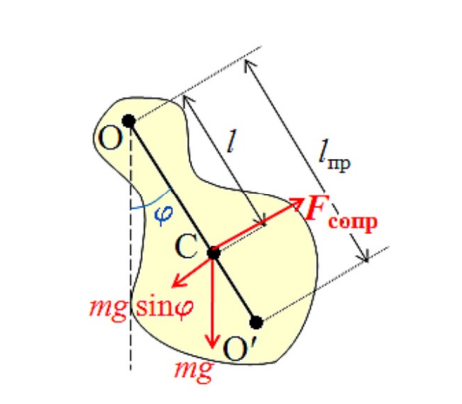
\includegraphics[width=0.5\textwidth]{1.png}
    \caption{Физический маятник. Ось качания (ось подвеса) проходит перпендикулярно рисунку в точке O, C - центр масс, O' центр качания}
\end{figure}



Уравнение свободных затухающих колебаний физического маятника

\begin{equation}
I \frac{d^2 \varphi}{dt^2} = -mg l\varphi - rl^2 \frac{d^2 \varphi}{dt^2}.
\end{equation}

Введем обозначения

\begin{equation}
\omega_0^2 = \frac{mgl}{I}, \beta = \frac{rl^2}{2I}
\end{equation}

где $\omega_0$ - циклическая частота собственных незатухающих колебаний маятника; $\beta$ - коэффициент затухания. Соответственно период колебаний маятника равен

\begin{equation}
T = 2\pi \sqrt{\frac{I}{mgl}}
\end{equation}

Приведенной длиной физического маятника называется длина математического маятника, имеющего такой же период колебаний, т. е.

\begin{equation}
    T = 2\pi \sqrt{\frac{I}{mgl}} = 2\pi \sqrt{\frac{l_{\text{пр}}}{g}}
\end{equation}

Учитывая, что момент инерции маятника относительно точки подвеса $I$ связан по теореме Штейнера с моментом инерции относительно центра масс $I_0$ соотношением $I = I_0 + ml^2$, из  получаем

\begin{equation}
    l_{\text{пр}} = \frac{I}{ml} = \frac{I_0}{ml} + l
\end{equation}

Точка O', находящаяся на расстоянии приведенной длины от оси подвеса, называется центром качания.

С учетом введенных обозначений уравнение  приводится к виду

\begin{equation}
\frac{d^2 \varphi}{dt^2} + 2\beta \frac{d \varphi}{dt} + \omega_0^2 \varphi = 0
\end{equation}

Решение уравнения (1) при $\beta < \omega_0$ имеет вид

\begin{equation}
\varphi = A_0 e^{-\beta t} cos(\omega t + \alpha_0)
\end{equation}

где $A_0$ - амплитуда в начальный момент времени; $\omega$ - циклическая частота затухающих колебаний, $\alpha_0$ - начальная фаза.

Таким образом, при наличии вязкого трения амплитуда колебаний убывает по экспоненциальному закону (рис. 2):

\begin{equation}
\varphi = A_0 e^{-\beta t}
\end{equation}

\begin{figure}[h]
\centering
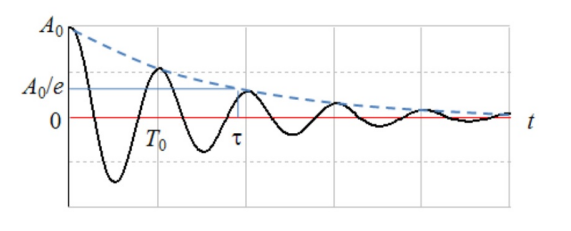
\includegraphics[width=0.5\textwidth]{2.png}
\caption{Затухающее колебание}
\end{figure}

За время $\tau = 1/\beta$ амплитуда убывает в $e = 2.72$ раз. Это время называется временем затухания. Логарифмируя уравнение 8, получаем, что

\begin{equation}
ln\frac{A}{A_0} = -\beta t
\end{equation}

т. е. график зависимости логарифма отношения амплитуд от времени представляет собой прямую, модуль коэффициента наклона которой равен коэффициенту затухания.

Вместо коэффициента затухания $\beta$, имеющего размерность частоты, бывает удобно использовать безразмерный параметр, который называется логарифмическим декрементом затухания:

\begin{equation}
\lambda = ln\frac{A(t)}{A(t + T)} = \beta T
\end{equation}

Логарифмический декремент затухания обратен числу колебаний за время затухания.

Кроме вязкого трения колебания маятника могут затухать из-за сухого трения в оси подвеса. Если при вязком трении момент силы трения пропорционален угловой скорости, то при сухом трении он постоянен. В этом случае у маятника по обе стороны от положения равновесия появляется зона застоя $\Delta \varphi_3$: если угол отклонения $|\varphi| < \Delta \varphi_3$, то момент силы трения уравновешивает момент силы тяжести, и маятник остается в покое.

Если угол отклонения превышает ширину зоны застоя, то пока маятник движется в одном направлении, постоянный момент сухого трения вызывает смещение средней точки колебаний к границе зоны застоя (в сторону, противоположную направлению вращения). При изменении направления движения после точки поворота средняя точка перескакивает к другой границе зоны застоя. Поэтому за один период колебаний амплитуда уменьшается на удвоенную ширину зоны застоя (т.е. на величину $4\Delta \varphi_3$). Амплитудные значения уменьшаются по линейному закону:

\[
A(t = nT) = A_0 - 4n\Delta \varphi_3
\]

Колебания прекращаются после конечного числа циклов. Рис. 3 иллюстрирует различие в затухании маятников с вязким и сухим трением.

\begin{figure}[h]
\centering
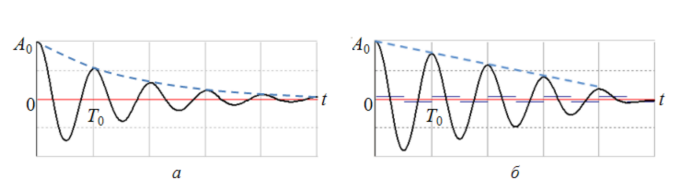
\includegraphics[width=0.8\textwidth]{3.png}
\caption{Затухание маятника с вязким (а) и сухим (б) трением}
\end{figure}


\section{\textbf{Экспериментальная установка}}



\begin{figure}[H]
\centering
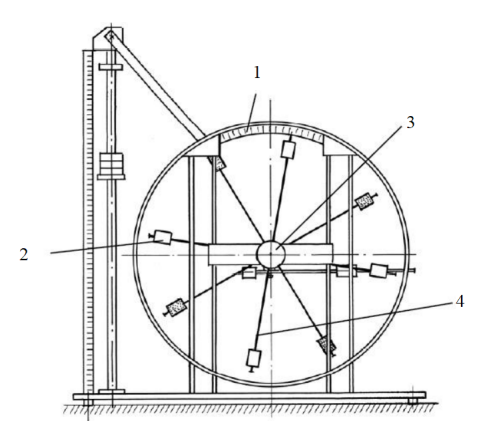
\includegraphics[width=0.5\textwidth]{1.05.4.png}
\caption{Стенд лаборатории механики (общий вид)}
\end{figure}


Работа выполняется на универсальном стенде (рис. 4).В состав установки входят:
\begin{enumerate}
    \item Шкала
    \item Груз
    \item Рукоятка сцепления
    \item Передняя крестовина
\end{enumerate}

В работе используется передняя крестовина. Угол отклонения маятника отсчитывается по шкале в угловых градусах. Время измеряется механическим или электронным секундомером.



\begin{table}[H]
\centering
\begin{tabular}{|l|c|c|c|}
\hline
Наименование & Диапазон измерений & Цена деления & Погрешность \\
\hline
Шкала & 0°- 60° & 1°/дел. & 1° \\
\hline
Секундомер & 0 -  & - & 0.005 c. \\
\hline
\end{tabular}
\caption{Характеристики средств измерения}
\end{table}
\begin{figure}[H]
\centering
\vspace{-0\textwidth}
\caption{Данные установки}
\end{figure}

\section{\textbf{Полученные данные}}

\begin{figure}[H]
\centering
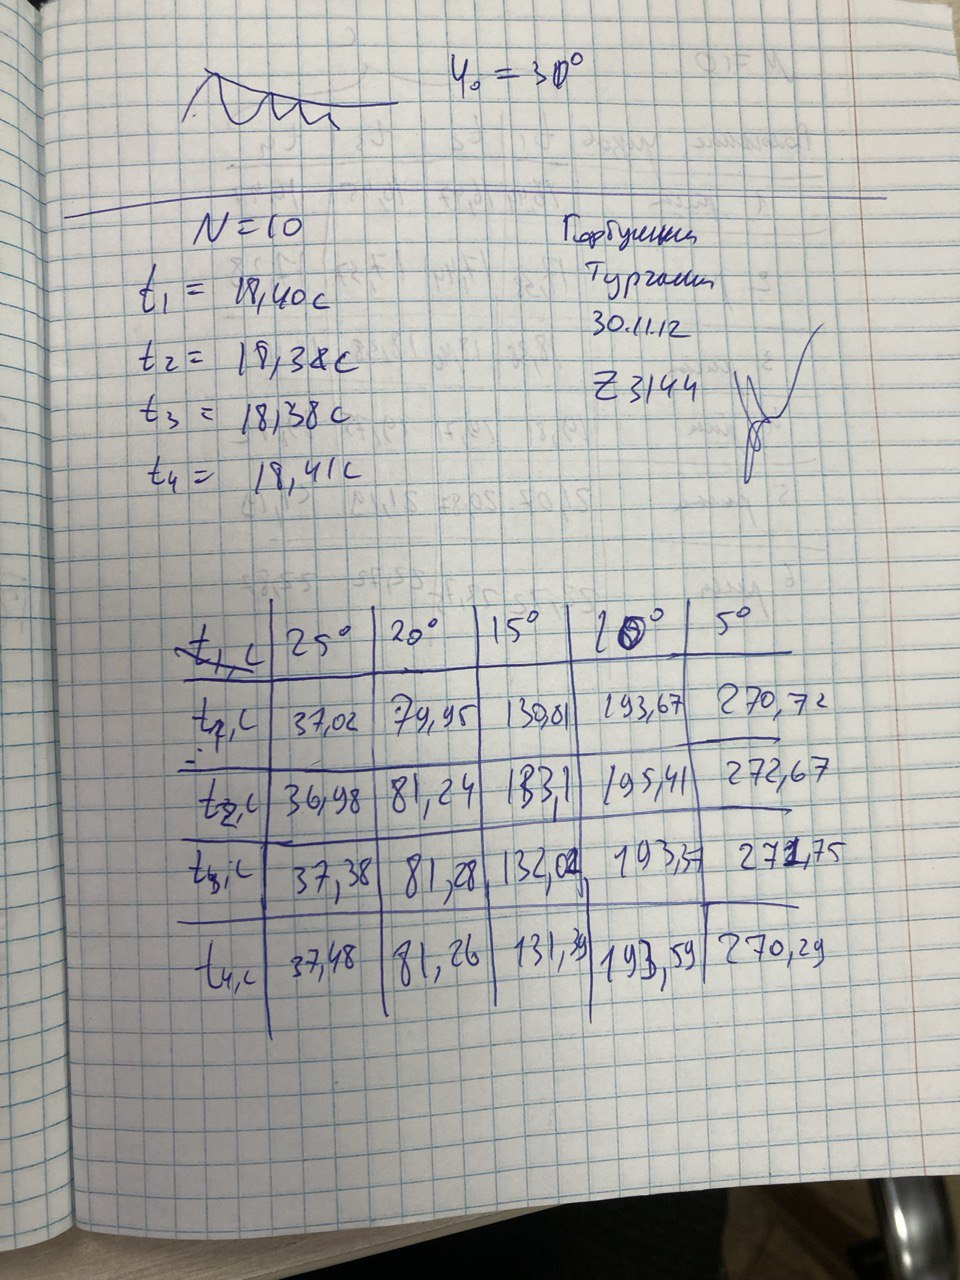
\includegraphics[width=0.3\textwidth]{data_1}
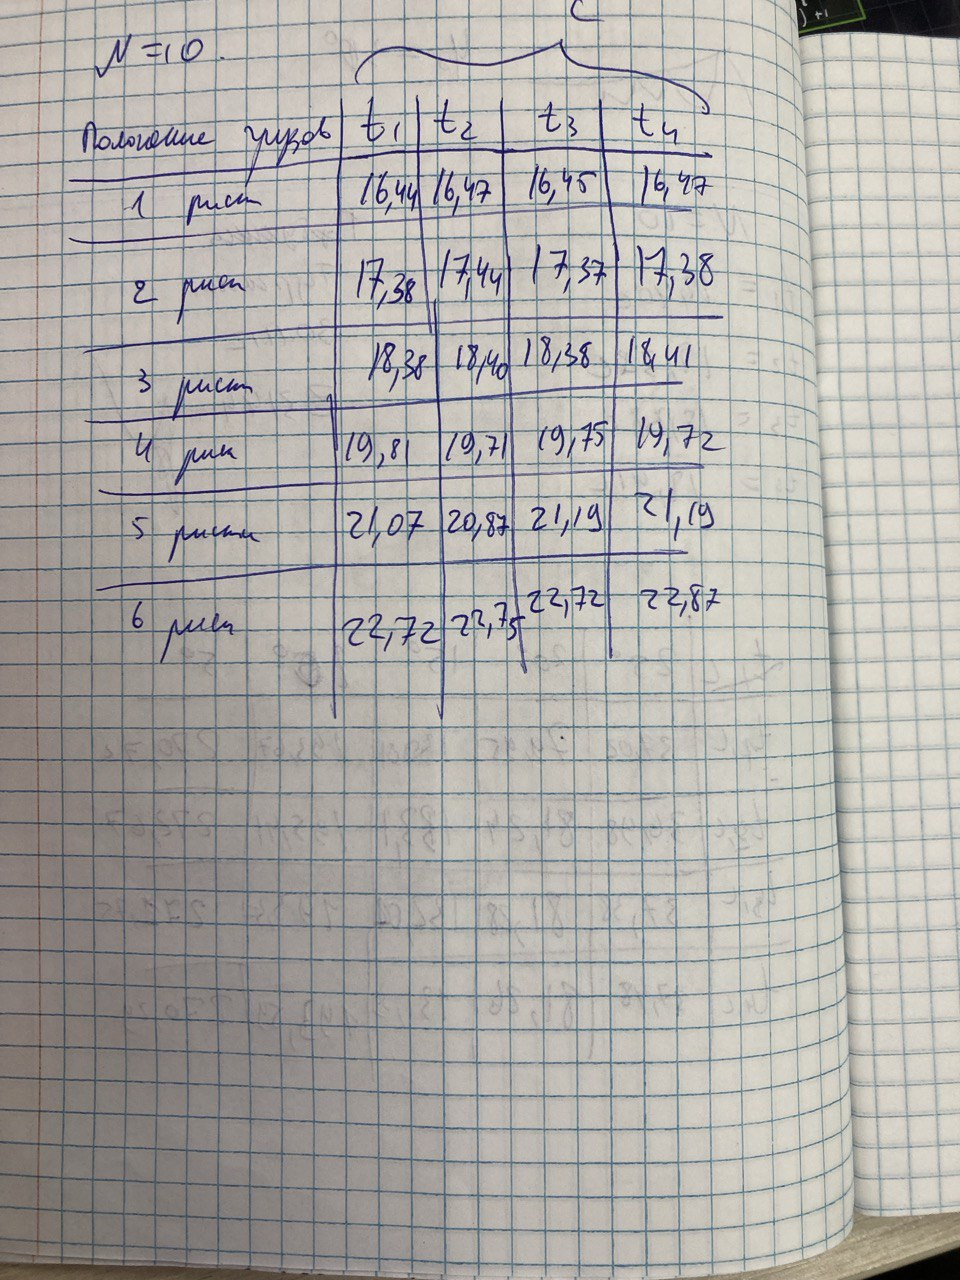
\includegraphics[width=0.3\textwidth]{data_2}
\end{figure}

\section{\textbf{Результаты}}


\begin{figure}[H]
\centering
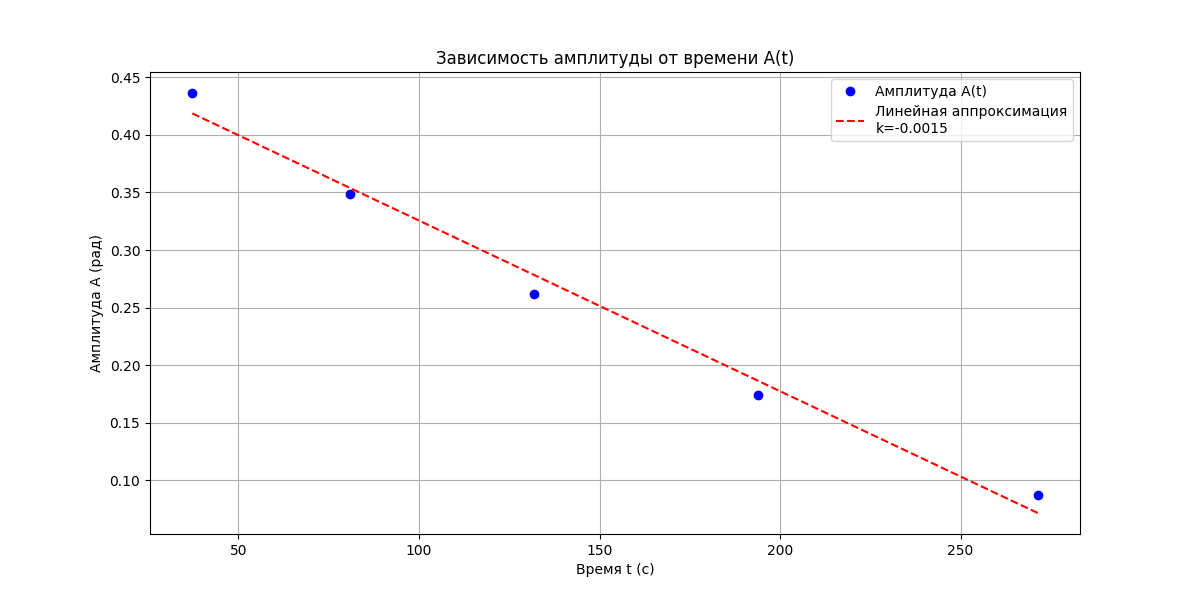
\includegraphics[width=0.5\textwidth]{4.png}
\end{figure}
Так как график больше похож на прямую, нежели на логарифм, то сухое трение преобладает\\
Ширина застоя: $\Delta \varphi_3 = 0.0002$ рад\\
Через 650 периодов колебания полностью прекратятся

\begin{figure}[H]
\centering
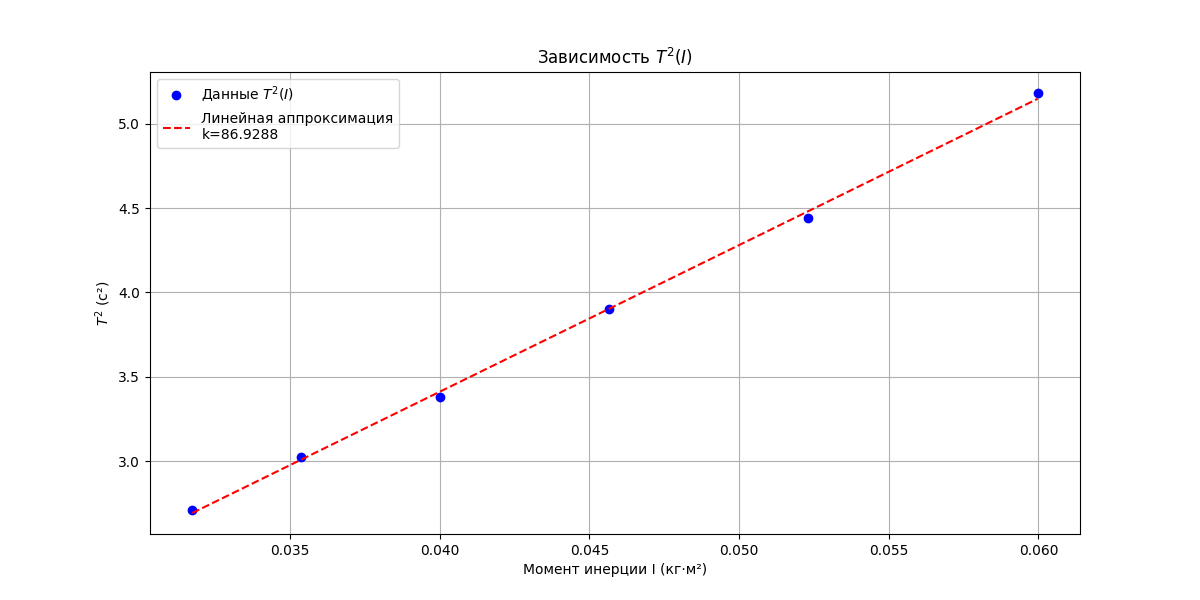
\includegraphics[width=0.5\textwidth]{5.png}
\end{figure}
Угловой коэфициент : $k = 86.93$\\
Тогда $ml=0.047$\\

Экспериментальные приведенные длины: 0.67,\, 0.75,\, 0.84,\, 0.97,\, 1.10,\, 1.29\\
Теоретические приведенные длины: 0.63,\, 0.70\, 0.79,\, 0.90,\, 1.03,\, 1.18\\


\section{\textbf{Заключение}}

\begin{enumerate}
\item Результат с приведенными длинами странный, так как экспериментальные длины получились больше чем теоретические. Из этого следует, что теоретический период должен быть меньше, хотя в теоретическом расчете учитывается вязкое трение, те петиод должен быть больше
\item Так же величины сильно отличаются, это может быть вызванно пренебрежением веса крестовины
\end{enumerate}

\end{document}
